\par Para esta etapa se busca calcular los tiempos de reverberación óptimos y diseñar el tratamiento acústico de la sala, teniendo en cuenta que la misma va a ser utilizada para palabra. Dicho tratamiento consta de la utilización de materiales fonoabsorbentes.\\

\par Para realizar este tratamiento, seguiremos los pasos indicados en la guía de informe del proyecto. En primer lugar, calculamos el tiempo de reverberación ($TR$) óptimo dado el volumen y el uso que se le dará a la sala (en nuestro caso, la palabra). Utilizando las curvas de \quotemarks{TR óptimos según el volumen y destino de uso} de \textit{Knudsen}, y gracias a las fórmulas provistas por la cátedra que modelan dichas curvas, podemos calcular los tiempos de reverberación óptimos como se muestra en el cuadro \ref{tab:ecuaciones_caluclo_TRoptimo}:

\begin{table}[h]
    \centering
    \begin{tabular}{|c|c|} \hline
        \textbf{Frecuencia [Hz]}  & \textbf{$TR_{optimos}$ [seg]} (V en $m^3$) \\ \hline
        125 & $TR_{125} = 0.41 + 0.26 \cdot log(V)$ \\ \hline
        250 & $TR_{250} = 0.32 + 0.21 \cdot log(V)$ \\ \hline
        >500 & $TR_{500} = 0.28 + 0.18 \cdot log(V)$ \\ \hline
    \end{tabular}
    \caption{Ecuaciones para cálculo de $TR_{optimos}$}
    \label{tab:ecuaciones_caluclo_TRoptimo}
\end{table}

\par Utilizando el dato del volumen de la sala que se tiene el cuadro \ref{tab:medidas_de_sala}, tenemos que $V = 346.8 m^3$. Por lo tanto los $TR_{optimos}$ obtenidos se presentan en el cuadro \ref{tab:TRoptimos_de_sala}. Como criterio de diseño, debemos considerar una banda de tolerancia para los valores obtenidos. Consideramos prudente una banda de tolerancia del 20\%:

\begin{table}[h]
    \centering
    \begin{tabular}{|c|c|} \hline
         $TR_{optimos}$ [seg] & $\pm Tolerancia$ [seg] \\ \hline 
         $TR_{125} = 1.0704$  & $0.2141$ \\ \hline
         $TR_{250} = 0.8534$  & $0.1707$\\ \hline
         $TR_{500} = 0.7372$  & $0.1474$ \\ \hline
    \end{tabular}
    \caption{Tiempos de reverberación óptimos para uso de Palabra para la sala estudiada}
    \label{tab:TRoptimos_de_sala}
\end{table}

\par En el gráfico \ref{fig:TR_optimosYtolerancia} se muestran los valores obtenidos junto con sus bandas de tolerancia para frecuencias de octavas comprendidas entre 125 y 4000Hz.


\begin{figure}[H]
	\centering
	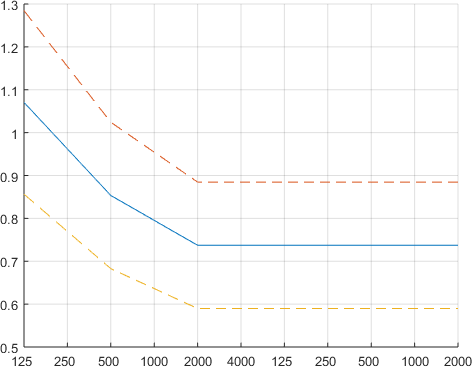
\includegraphics[width=1\textwidth]{./img/TR_optimosYtolerancia.png}
	\caption{Gráfico de valores de $TR_{optimo}$ y sus bandas de tolerancia LO TENGO QUE CAMBIAR}
	\label{fig:TR_optimosYtolerancia}
\end{figure}

\par A continuación seleccionamos los materiales con que estarán construidas las superficies interiores del recinto (piso, techo, paredes, puertas) y el tipo y cantidad de muebles. Para esto, consideramos las recomendaciones de diseño acústico para aulas y salas de conferencias del \quotemarks{\textit{Código Técnico de la Edificación}} (\textbf{CTE} España), donde se recomienda material absorbente acústico en toda la superficie del techo, una pared detras del orador reflectante y las demás absorbentes. Los materiales para el recinto se muestran en el cuadro \ref{tab:materiales_construccion_recinto}.

\begin{table}[h]
    \centering
    \begin{tabular}{|c|c|c||c|c|c|c|c|c|} \hline
        Tipo &  Material elegido &Sup./Cant. & \multicolumn{6}{|c|}{Coeficiente $\alpha$, Área equivalente [$m^2$]} \\ \hline
        \multicolumn{3}{|c|}{Frecuencia [Hz]:} & 125 & 250 & 500 & 1000 & 2000 & 4000 \\ \hline \hline
        Piso & Baldosa enlozada & 13.9$m^2$ & 0.01 & 0.02 & 0.02 & 0.03 & 0.03 & 0.04 \\ \hline
        Paredes (frente orador) & Ladrillo Pintado & 118.66 $m^2$ & 0.01 & 0.01 & 0.02 & 0.02 & 0.02 & 0.02 \\ \hline
        Pared (detrás orador) & Ladrillo pintado & 47.26 $m^2$ & 0.01 & 0.01 & 0.02 & 0.02 & 0.02 & 0.02 \\ \hline
        Techo & Enlucido &13.9$m^2$ & 0.01 & 0.03 & 0.04 & 0.05 & 0.08 & 0.17 \\ \hline
        Puertas (1.5m x 2m) & Madera maciza & 3 $\times$ 3$m^2$ & 0.05 & 0.11 & 0.10 & 0.09 & 0.08 &  0.10 \\ \hline \hline
        Butacas & Tapizado 2 & (CANT) & 0.12 & 0.20 & 0.28 & 0.30 & 0.31 & 0.37 \\ \hline
        Butaca & Madera & 1 & 0.01 & 0.02 & 0.02 & 0.04 & 0.04 & 0.04 \\ \hline
    \end{tabular}
    \caption{Materiales y objetos para la construcción del recinto}
    \label{tab:materiales_construccion_recinto}
\end{table}

\par Para las paredes en donde el orador se enfrenta desde el escenario, la recomendación indica que deben ponerse materiales absorbentes, por lo tanto, se eligieron las paredes de papel pintado cuyos coeficientes de absorción sonora era más alta que los demás materiales. Lo mismo para el piso y techo se siguió el mismo criterio. Luego, como buscamos una pared reflejante detrás del orador, se optó por construir dicha pared con ladrillo pintado.

\par Se esperá cumplir con los tiempos de reverberación óptimos para una  \textcolor{red}{ocupación del \textbf{75\%}}.\\

\par A continuación, procedemos con calcular el tiempo de reverberación inicial correspondiente a la sala con muebles y con el estado de ocupación definido, para las octavas con frecuencias centrales comprendidas entre 125 y 4000Hz.

